\documentclass[a4paper,12pt]{article}

% Package for Unicode support
\usepackage[utf8]{inputenc}
\usepackage{float}
\usepackage{placeins}
% Language and font encoding
\usepackage[utf8]{inputenc}
\usepackage[greek,english]{babel} % Add Greek and English language support
\usepackage{alphabeta} % Allows you to switch between Greek and Latin alphabets
\usepackage{amsmath}
% Geometry package for page margins
\usepackage{geometry}
\geometry{
 a4paper,
 total={170mm,257mm},
 left=25mm,
 right=25mm,
 top=25mm,
 bottom=25mm
}

% For math symbols and equations
\usepackage{amsmath}
\usepackage{siunitx}
\usepackage{caption}
\usepackage{booktabs}

% Graphicx for including images
\usepackage{graphicx}
\graphicspath{{figures/}}

% Hyperlink support with hidden links
\usepackage[hidelinks]{hyperref}


% Package for professional tables
\usepackage{booktabs}

% Package for fancy header and footer
\usepackage{fancyhdr}
\pagestyle{fancy}
\fancyhf{}
\fancyhead[L]{ΠΤΣΑΕ} % Module name in header
\fancyhead[R]{\leftmark} % Section title in header
\fancyfoot[C]{\thepage} % Page number in the footer

% For including code snippets
\usepackage{listings}
\lstset{
    basicstyle=\ttfamily,
    breaklines=true
}

% Title page formatting
\title{
    \vspace{2cm}
    \textbf{Έλεγχος Drone}\\
    \large Μάθημα: Προχωρημένες Τεχνικές Συστημάτων Αυτομάτου Ελέγχου\\
    \vspace{1cm}
}
\author{
    Στυλιανός Μπούλιαρης - Μαλατέστας\\
    ΑΜ: 03119214\\
    \vspace{0.5cm}
    Εθνικό Μετσόβιο Πολυτεχνείο\\
    Σχολή Ηλεκτρολόγων Μηχανικών \& Μηχανικών Υπολογιστών
}
\date{\selectlanguage{greek}\today}

% Begin Document
\begin{document}

% Title page
\maketitle
\thispagestyle{empty}
\newpage

% Table of contents
\tableofcontents
\newpage

% Section 1: Introduction
\section{Εισαγωγή}
Στην άσκηση αυτή θα ασχοληθούμε με τον έλεγχο ενός Drone (quadrotor). Συγκεκριμένα θα δοκιμάσουμε διαφορετικούς τρόπους ελέγχου, όπως PID, Cascaded PID και έλεγχο στο χώρο κατάστασης χρησιμοποιώντας LQR. Στο τέλος θα δοκιμάσουμε να δώσουμε μια πορεία στο Drone με τους ελεγκτές που έχουμε σχεδιάσει, και θα δούμε πως ανταποκρίνεται το σύστημα μας. Το Drone μας φαίνεται στο παρακάτω σχήμα:
% Insert an image
\begin{figure}[h] % 'h' places the image approximately where it appears in the code
    \centering
    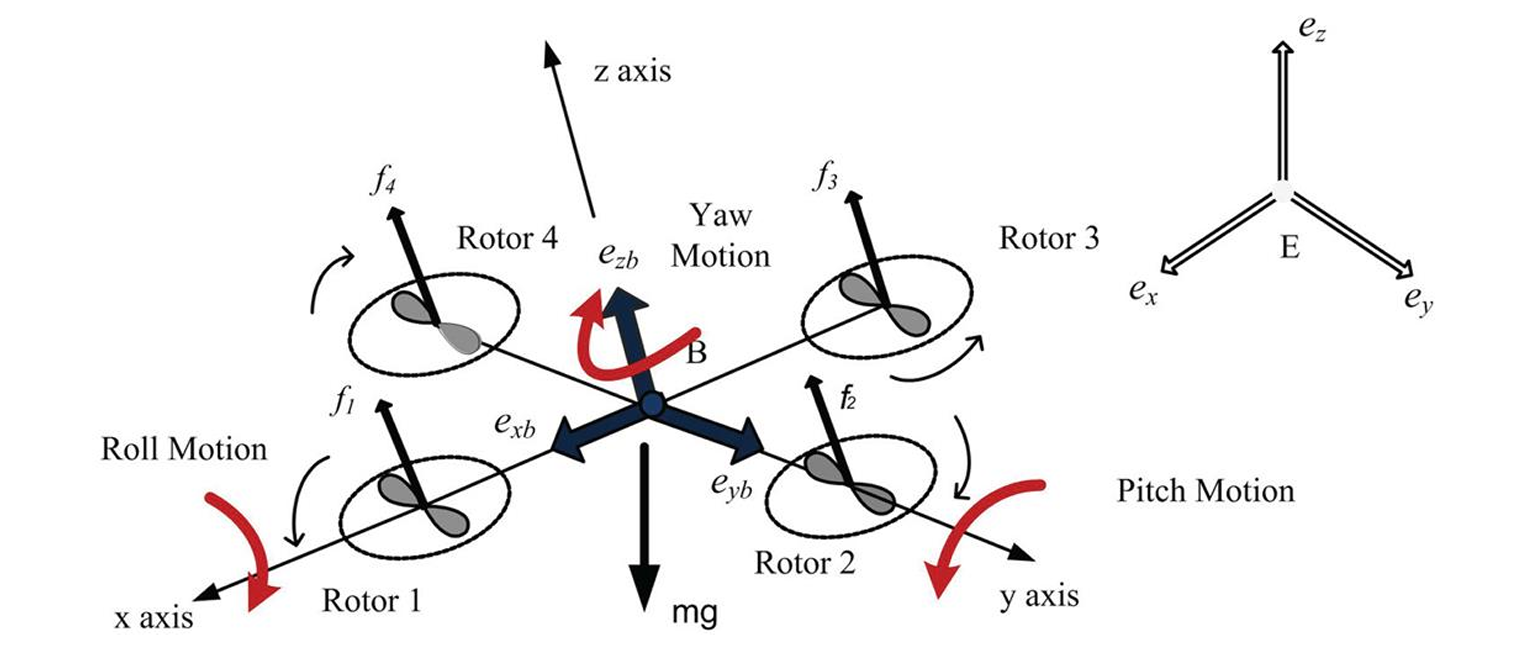
\includegraphics[width=0.9\textwidth]{DroneSchematic.png} % Specify image file and width
    \caption{Quadrotor Drone System} % Image caption
    \label{fig:DroneSchematic} % Label for referencing the image
\end{figure}
\newline
To drone μας έχει 6 βαθμούς ελευθερίας, 3 στροφές roll, pitch, yaw ($φ, \theta, ψ$) και 3 μεταφορές ($x, y, z$). Προφανώς η ταχύτητα περιστροφής των κινητήρων (άρα και το lift force που δημιουργεί ο κάθε κινητήρας), επηρεάζουν τις μεταβλητές κατάστασης του drone που μόλις περιγράψαμε.

\newpage







% Section 2: Theory
\section{Μοντελοποίηση Συστήματος}
\subsection{Περιγραφή Περιστροφικής Κίνησης}
Το drone έχει 4 έλικες. Οι δύο γυρνούν σύμφωνα με τη φορά των δεικτών του ρολογιού (οι 
έλικες από τον άξονα που περνάει ο x’ άξονας) και οι άλλοι δύο αντίστροφα. Έτσι σε 
λειτουργία hovering, που μένει σταθερό σε ένα σημείο, η συνολική στροφορμή των ελίκων 
είναι 0. Η ώθηση που δίνει ο κάθε έλικας ($i=1,2,3,4$) είναι ανάλογη του τετραγώνου της 
γωνιακής ταχύτητάς του και δίνεται από τη σχέση:
\begin{equation}
    f_i = b\Omega_i^2
\end{equation}
Για να στύψει το drone γύρω από τον άξονα των x (κίνηση roll, αλλαγή της γωνίας φ) αρχικά 
ελαττώνεται η ταχύτητα έλικα 2 και αυξάνει του 4, κάτι που δημιουργεί μια ροπή γύρω από 
τον άξονα των x, η οποία στη συνέχεια δημιουργεί μια γωνιακή ταχύτητα (προφανώς για να 
σταματήσει αυτή η γωνιακή κίνηση θα χρειαστεί μια αντίθετη ροπή). Αντίστοιχα η στροφή 
γύρω από τον y άξονα επιτυγχάνεται με τη διαφορά των ταχυτήτων των ελίκων 1, 3. Η 
περιστροφή γύρω από τον z άξονα γίνεται μέσω της αύξησης της ταχύτητας δύο 
αντιδιαμετρικών ελίκων και την μείωση στο άλλο ζευγάρι (η ροπή επιτυγχάνεται μέσω της 
αντίστασης drag στην κίνηση των ελίκων).  
\subsection{Περιγραφή Μεταφορικής Κίνησης}
Προκειμένου να κινηθεί το drone στον άξονα z, θα πρέπει η συνολική δύναμη στον άξονα αυτόν να είναι μεγαλύτερη του βάρους. Η δύναμη περιγράφεται από τη σχέση:
\begin{equation}
    U_1 = b(\Omega_1^2+\Omega_2^2+\Omega_3^2+\Omega_4^2)
\end{equation}
Για να υπάρξει κίνηση στους άξονες x και y, πρώτα το drone πρέπει να στραφεί γύρω από τους άξονες y (pitch) και x (roll) αντίστοιχα, προκειμένου να εμφανιστεί μια συνιστώσα της συνολικής δύναμης $U_1$ στον άξονα που θέλουμε να υπάρξει κίνηση. Επομένως οι παρακάτω σχέσεις εκφράζουν:
\begin{equation}
    U_2 = b(\Omega_4^2 - \Omega_2^2),  \quad \textrm{Το $U_2$ ελέγχει την κίνηση στον άξονα x}
\end{equation}

\begin{equation}
    U_3 = b(\Omega_3^2 - \Omega_1^2),  \quad \textrm{Το $U_3$ ελέγχει την κίνηση στον άξονα y}
\end{equation}

\begin{equation}
    U_4 = d(\Omega_1^2+\Omega_3^2-\Omega_2^2-\Omega_4^2),  \quad \textrm{Το $U_4$ ελέγχει την στροφή γύρω από z}
\end{equation}
\newline
Σημειώστε ότι τα $U_1,U_2,U_3$ εξαρτώνται από το συντελεστή άνωσης b ενώ το $U_4$ από το 
συντελεστή αντίστασης d.
\newpage
\subsection{Μαθηματική Μοντελοποίηση στο Χώρο Κατάστασης}
Οι μεταβλητές κατάστασης που χρειαζόμαστε για να περιγράψουμε το σύστημα δεν είναι άλλες παρά τις γωνίες Euler $φ, \theta, \psi$ γύρω από τους άξονες, καθώς και οι μεταφορές $x, y, z$ στους άξονες αυτούς. Οι εξισώσεις κατάστασης για τις στροφικές κινήσεις είναι οι εξής:
\begin{equation}
    \Ddot{\phi} = \dot{\theta}\dot{\psi}[\frac{I_{yy}-I_{zz}}{I_{xx}}] + \frac{1}{I_{xx}}U_2
\end{equation}

\begin{equation}
    \Ddot{\theta} = \dot{\phi}\dot{\psi}[\frac{I_{yy}-I_{xx}}{I_{yy}}] + \frac{1}{I_{yy}}U_3
\end{equation}

\begin{equation}
    \Ddot{\psi} = \dot{\theta}\dot{\phi}[\frac{I_{xx}-I_{yy}}{I_{zz}}] + \frac{1}{I_{zz}}U_4
\end{equation}
\newline
Η κίνηση στους άξονες $x, y, z$ δίνεται από τις εξισώσεις:
\begin{equation}
    \Ddot{x} = (c_{\phi}s_{\theta}c_{\psi} + s_{\phi}s_{\psi})\frac{1}{m}U_1
\end{equation}

\begin{equation}
    \Ddot{y} = (-c_{\phi}s_{\theta}s_{\psi} + s_{\phi}c_{\psi})\frac{1}{m}U_1
\end{equation}

\begin{equation}
    \Ddot{z} = -g +(c_{\phi}c_{\theta})\frac{1}{m}U_1
\end{equation}
\newline
\noindent
Στις παραπάνω εξισώσεις, οι όροι $c_{i}, s_{i}$ αποτελούν συντομογραφίες για $cos(i), sin(i)$. Για την συνέχεια της άσκησης, παίρνουμε τις τιμές των μεταβλητών που βρίσκονται στις παραπάνω εξισώσεις σύμφωνα με τον πίνακα $(1)$. Θα θεωρήσουμε επιπλέον πως κάθε έλικα μπορεί να περιστραφεί με μέγιστη ταχύτητα $\Omega_{max} = 15000 RPM$

\begin{table}[h!]
\centering
\caption{Physical parameters of the quadrotor system.}
\begin{tabular}{lll}
\toprule
\textbf{Parameter} & \textbf{Symbol} & \textbf{Value} \\
\midrule
Total weight of the vehicle         & \( m \)   & 0.800 kg \\
Gravitational acceleration          & \( g \)   & 9.81 
\(\si{\meter\per\second\squared}\) \\
Arm length of the vehicle           & \( l \)   & 0.3 m \\
Moment of inertia along x-axis      & \( I_{xx} \) & \( 15.67 \times 10^{-3} \, \si{\kilogram\meter\squared} \) \\
Moment of inertia along y-axis      & \( I_{yy} \) & \( 15.67 \times 10^{-3} \, \si{\kilogram\meter\squared} \) \\
Moment of inertia along z-axis      & \( I_{zz} \) & \( 28.34 \times 10^{-3} \, \si{\kilogram\meter\squared} \) \\
Thrust factor                       & \( b \)   & \( 192.32 \times 10^{-7} \, \si{\newton\second\squared} \) \\
Drag factor                         & \( d \)   & \( 4.003 \times 10^{-7} \, \si{\newton\meter\second\squared} \) \\
\bottomrule
\end{tabular}
\end{table}
\newpage









% Section 3 Control
\section{Cascaded PID Έλεγχος}
\subsection{Εξάλειψη γωνιών $\phi, \theta$ και διατήρηση του drone σε σταθερό ύψος}\label{3.1}
Στόχος μας είναι να σταθεροποιήσουμε τις γωνίες $\phi, \theta$ στο $0$ όσο διατηρούμε το ύψος του drone σε συγκεκριμένη επιθυμητή τιμή. Επιλέξαμε σαν αρχικές συνθήκες:
\begin{table}[h!]
\centering
\caption{Initial Conditions}
\begin{tabular}{|c|c|c|}
\hline
\textbf{Variable Name} & \textbf{Symbol} & \textbf{Value} \\ \hline
Initial $\phi$ & $\phi_0$ & $0.02 rad$ \\ \hline
Initial $\theta$ & $\theta_0$  & $0.02 rad$ \\ \hline
Initial $z$ & $z_0$  & $0 m$ \\ \hline
\end{tabular}
\end{table}

\noindent
Κατασκευάζουμε λοιπόν έναν PID ελεγκτή για κάθε μία από τις εισόδους $U_1, U_2, U_3$, καθώς αυτές είναι υπεύθυνες για τις κινήσεις που θέλουμε να ελέγξουμε. Μετά από δοκιμές, καταλήγουμε πως τα ιδανικά κέρδη για τους ελεγκτές είναι: 
\begin{equation}
    [K_p = 1, K_i = 0.5, K_d = 4],   \quad \textrm{Για το $U_1$}
\end{equation}
\begin{equation}
    [K_p = 2, K_i = 0, K_d = 0.35],   \quad \textrm{Για το $U_2, U_3$}
\end{equation}
\noindent
Παρακάτω βλέπουμε την απόκριση του drone με τη χρήση των παραπάνω ελεγκτών, όταν θέτουμε σαν επιθυμητή τιμή για το $z = 1m$
\begin{figure}[h!] % 'h' places the image approximately where it appears in the code
    \centering
    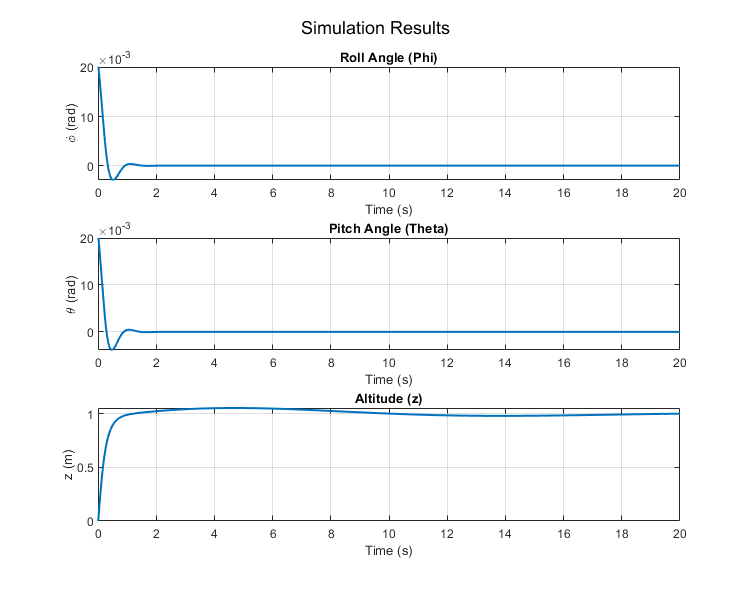
\includegraphics[width=0.8\textwidth]{DroneResponsePID.png} % Specify image file and width
    \caption{Response with gains specified in $(12), (13), (14)$ for $z_{d} = 1$} % Image caption
    \label{fig:DroneResponsePID} % Label for referencing the image
\end{figure}
\newline
Βλέπουμε λοιπόν πως το σύστημα μας αποκρίνεται αρκετά γρήγορα, και σταθεροποιείται στη μόνιμη κατάσταση όπως θέλουμε. 
\subsection{Έλεγχος $x, y, z$ σε επιθυμητές τιμές, χρησιμοποιώντας Cascaded PID}\label{3.2}
Στόχος τώρα είναι το drone μας να φτάνει σε ένα επιθυμητό σημείο, με συντεταγμένες $x, y, z$ στον καρτεσιανό χώρο. Για να το κάνουμε αυτό, θα σχεδιάσουμε 2 Cascaded PID ελεγκτές για τη θέση $x$ και $y$ και θα χρησιμοποιήσουμε τον ελεγκτή που σχεδιάσαμε προηγουμένως για τη σταθεροποίηση του drone σε συγκεκριμένο z. Οι συντεταγμένες του σημείου που θέλουμε να φτάσουμε είναι:
 \begin{table}[h!]
\centering
\caption{Desired Coordinates}
\begin{tabular}{|c|c|c|}
\hline
\textbf{Variable Name} & \textbf{Symbol} & \textbf{Value} \\ \hline
Desired $x$ & $x_d$  & $1m$ \\ \hline
Desired $y$ & $y_d$  & $4m$ \\ \hline
Desired $z$ & $z_d$  & $4m$ \\ \hline
\end{tabular}
\end{table}
\begin{figure}[h!] % 'h' places the image approximately where it appears in the code
    \centering
    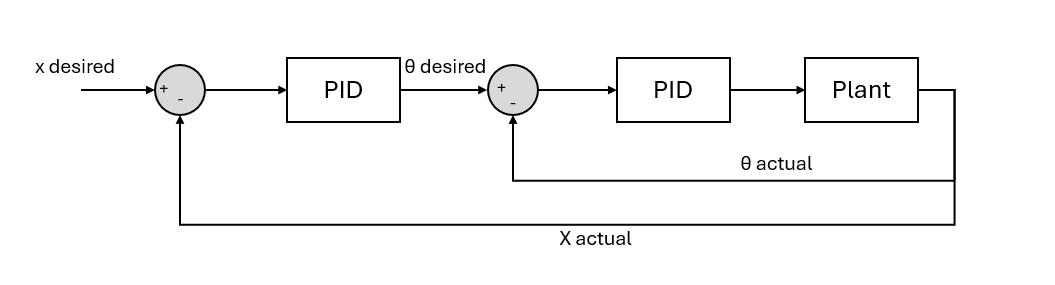
\includegraphics[width=1\textwidth]{CascadedControllerBlockDiagram.png} % Specify image file and width
    \caption{Block diagram of Cascaded PID for $\theta$} % Image caption
    \label{fig:CascadedBlockDiagram} % Label for referencing the image
\end{figure}

\noindent
Κρίθηκε σκόπιμο να περιμένουμε να σταθεροποιηθεί το drone στο ύψος στο οποίο θέλουμε πρώτα, και μετά να δώσουμε εντολή να μεταβεί στα επιθυμητά $x$ και $y$. Μετά από δοκιμές τα gains που χρησιμοποιήθηκαν στους Cascaded PID ελεγκτές είναι:
\begin{equation}
    [K_p = 1, K_i = 0, K_d = 0.7],   \quad \textrm{Για τον υπολογισμό desired γωνίας}
\end{equation}

\begin{equation}
    [K_p = 2.95, K_i = 0.5, K_d = 2.6],   \quad \textrm{Για τον έλεγχο των κινητήρων}
\end{equation}

\noindent
Επιπλέον είναι σημαντικό να αναφέρουμε πως ο απευθείας έλεγχος των γωνιών $\phi, \theta$ χρησιμοποιώντας τις global συντεταγμένες $x$ και $y$ δεν λειτουργεί, καθώς ακόμη δεν κάνουμε έλεγχο στη γωνία $\psi$, επομένως, όταν στρέφεται το drone, οι άξονες του παύουν να συμπίπτουν με το αδρανειακό σύστημα global σύστημα αναφοράς. 
\newline
\newline
Ο μετασχηματισμός στο σύστημα αναφοράς του drone γίνεται ως εξής:
\begin{equation}
    x_{drone} = xcos(\psi)+ysin(\psi)
\end{equation}

\begin{equation}
    y_{drone} = ycos(\psi)-xsin(\psi)
\end{equation}
\newpage
\noindent
Παρακάτω βλέπουμε την απόκριση του drone με τη χρήση του συστήματος ελέγχου που περιγράψαμε. Σημαντικό είναι να αναφέρουμε ότι έχουμε περιορίσει τις εξόδους των PID που υπολογίζουν τις επιθυμητές γωνίες ανάλογα με την απόκλιση της θέσης στο διάστημα $\phi,\theta \in [-15, 15]$, με στόχο την αποφυγή μεγάλων target γωνιών, που πιθανώς να έστελνε σε αστάθεια το σύστημα.
\begin{figure}[h!] % 'h' places the image approximately where it appears in the code
    \centering
    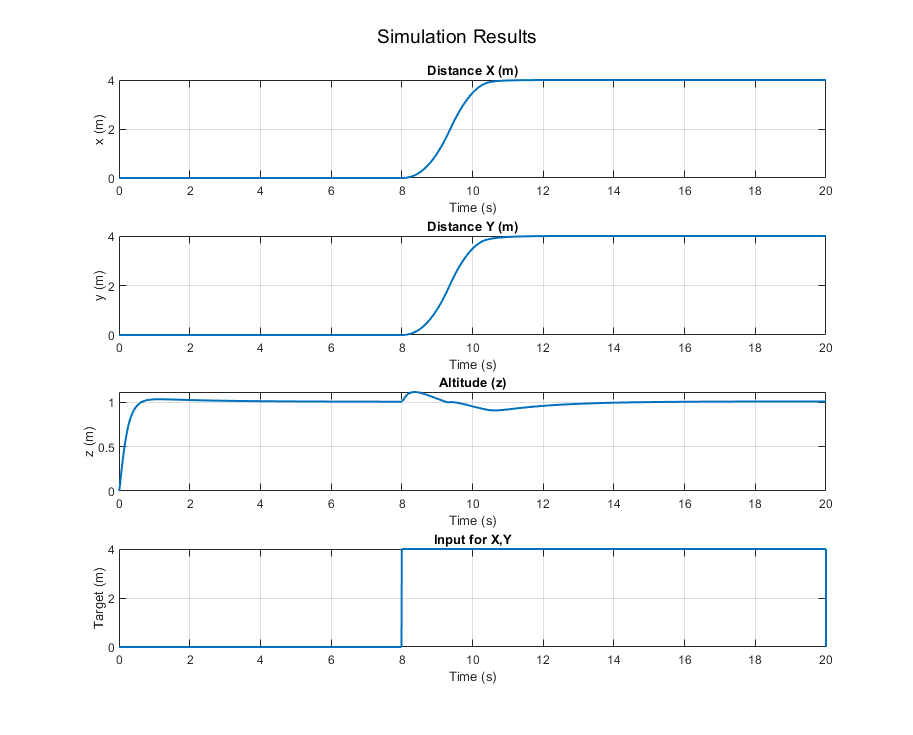
\includegraphics[width=1\textwidth]{DroneResponseCPID_disp.png} % Specify image file and width
    \caption{Drone position \& Controller input } % Image caption
    \label{fig:DroneResponseCPID_disp} % Label for referencing the image
\end{figure}
\newline
Παρατηρούμε πως όταν το drone αρχίζει να κινείται στους άξονες $x$ και $y$ το ύψος κάνει overshoot που δεν είναι έυκολο να γίνει compensated γρήγορα, καθώς δε μπορούμε να ασκήσουμε δύναμη προς τα κάτω, πάρα μόνο, να μειώσουμε την άνωση, αφήνοντας τη βαρύτητα να επαναφέρει το overshoot. Ωστώσο παρατηρήσαμε πως το συγκεκριμένο overshoot κατά την αρχική επιτάχυνση καθώς και το undershoot στην επιβράδυνση συνδέονται άμεσα με τα όρια των γωνιών που επιτρέπουμε στο drone. Έτσι τα όρια γωνιών που συζητήσαμε παραπάνω, αποτελούν ένα συμβιβασμό μεταξύ ταχύτητας απόκρισης και σφάλματος στο θέση $z$
\newline
\newline
Στη συνέχεια βλέπουμε την απόκριση γωνιών του drone. Στην αρχή ο στόχος είναι να σταθεροποιηθεί σε ύψος $z = 1$, που δεν επηρεάζει τις γωνίες. Στα 8 δευτερόλεπτα που το drone έχει πλέον σταθεροποιηθεί ξεκινάει να ακολουθεί τους στόχους για τις συντεταγμένες $x$ και $y$. Περιμένουμε λοιπόν να παρατηρήσουμε μεταβολή των γωνιών $\phi, \theta$.
\begin{figure}[h!] % 'h' places the image approximately where it appears in the code
    \centering
    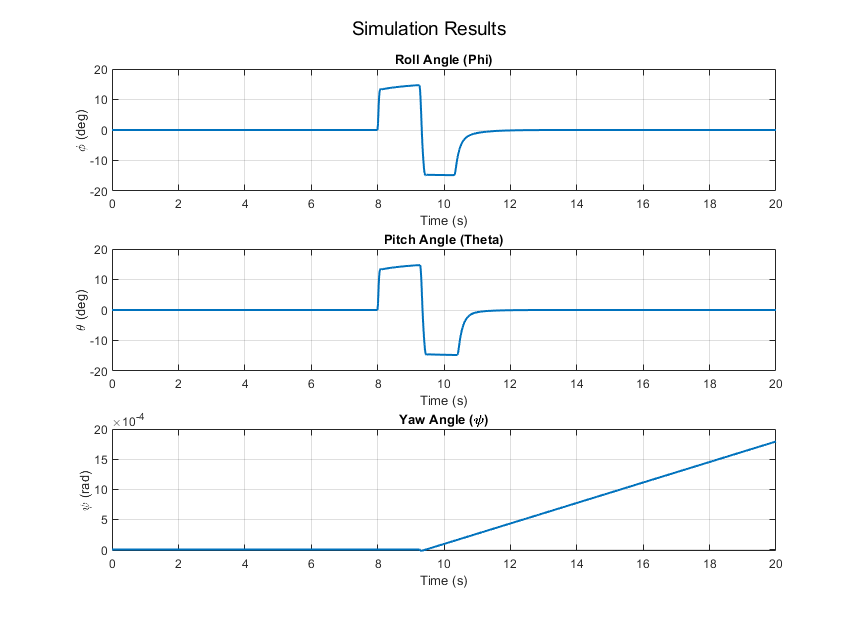
\includegraphics[width=1\textwidth]{DroneResponseCPID.png} % Specify image file and width
    \caption{Drone Euler angles } % Image caption
    \label{fig:DroneResponseCPID} % Label for referencing the image
\end{figure}
\newpage
\noindent
Παρατηρούμε πως η γωνία yaw ($\psi$) δεν μεταβάλεται και παραμένει πρακτικά σταθερή, παρά το γεγονός ότι δε την ελέγχουμε. Αυτό οφείλεται στο ότι οι στόχοι και οι ελεγκτές για τις γωνίες $\phi, \theta$ είναι ίδιοι, επομένως δίνοντας την ίδια εντολή ταχύτητας, οι ροπές yaw ακυρώνονται. Τα διαγράμματα ταχυτήτων κάθε έλικα φαίνονται στο διάγραμμα \ref{fig:Drone_Angular_Velocities}.
\newline
\newline
Αξίζει επίσης να αναφέρουμε πως παρότι χρησιμοποιήθηκε ο ίδιος ελεγκτής όπως και στο \ref{3.1}, τα κέρδη του χρειάστηκαν προσαρμογή, ώστε να μειωθεί το μέγιστο σφάλμα στην μεταβατική κατάσταση. Τα νέα κέρδη φαίνονται παρακάτω:
\begin{equation}
    [K_p = 2, K_i = 0.1, K_d = 4.4],   \quad \textrm{Για το $U_1$}
\end{equation}
\begin{figure}[h!] % 'h' places the image approximately where it appears in the code
    \centering
    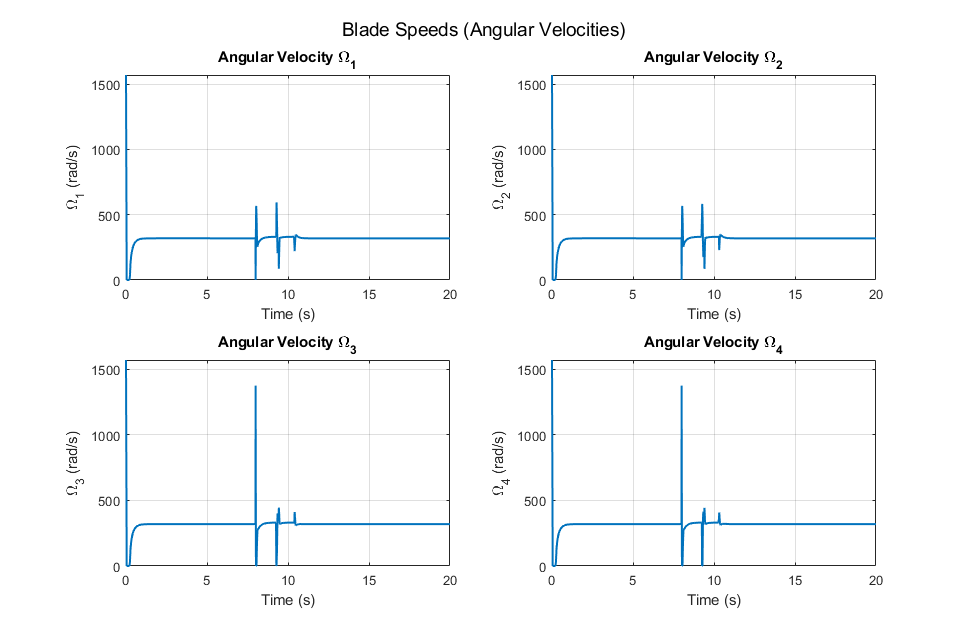
\includegraphics[width=1\textwidth]{Drone_Angular_Velocities.png} % Specify image file and width
    \caption{Drone angular velocities } % Image caption
    \label{fig:Drone_Angular_Velocities_plot} % Label for referencing the image
\end{figure}
\newpage
\subsection{Έλεγχος $x, y, z$ καθώς και $\psi$ σε επιθυμητές τιμές, χρησιμοποιώντας Cascaded PID}
Στόχος τώρα είναι να κάνουμε τον έλεγχο του ερωτήματος \ref{3.2} ενώ ταυτόχρονα ελέγχουμε και τη γωνία yaw ($\psi$). Για να το πετύχουμε αυτό θα κρατήσουμε το controller concept που περιγράφηκε προηγουμένως, και θα υλοποιήσουμε εκ νέου έναν απλό PID που θα ελέγχει το yaw. Στην περίπτωση που χρειαστεί, θα γίνουν και αλλαγές στους άλλους ελεγκτές για να βελτιωθεί η συνδυασμένη απόδοση του συστήματος.
\newline
\newline
Μετά από δοκιμές καταλήγουμε στα παρακάτω κέρδη για τους ελεγκτές. Παρατηρούμε πως χρειάστηκαν πολύ μικρές αλλαγές και όχι σε όλους τους ελεγκτές. Ακόμη, για τον έλεγχο της yaw γωνίας χρησιμοποιήθηκε ο ίδιος ελεγκτής που είναι υπεύθυνος για τον έλεγχο των κινητήρων στους Cascaded PID.
\begin{equation}
    [K_p = 2, K_i = 0.1, K_d = 4.4],   \quad \textrm{Για το $U_1$}
\end{equation}

\begin{equation}
    [K_p = 1, K_i = 0, K_d = 1.05],   \quad \textrm{Για τον υπολογισμό desired γωνίας}
\end{equation}

\begin{equation}
    [K_p = 2.95, K_i = 0.5, K_d = 2.6],   \quad \textrm{Για τον έλεγχο των κινητήρων}
\end{equation}

\begin{equation}
    [K_p = 2.95, K_i = 0.5, K_d = 2.6],   \quad \textrm{Για το $U_4$}
\end{equation}

\newpage
\noindent
Παρακάτω φαίνεται η απόκριση του συστήματος. Αξίζει να σημειωθεί πως αυτή τη τώρα οι στόχοι για την θέση $x$ και $y$, ορίζονται με χρονική διαφορά 1 δευτερόλεπτο, με σκοπό να δυσκολέψει ακόμη περισσότερο ο ρόλος του ελεγκτή του yaw. 
\begin{figure}[h!] % 'h' places the image approximately where it appears in the code
    \centering
    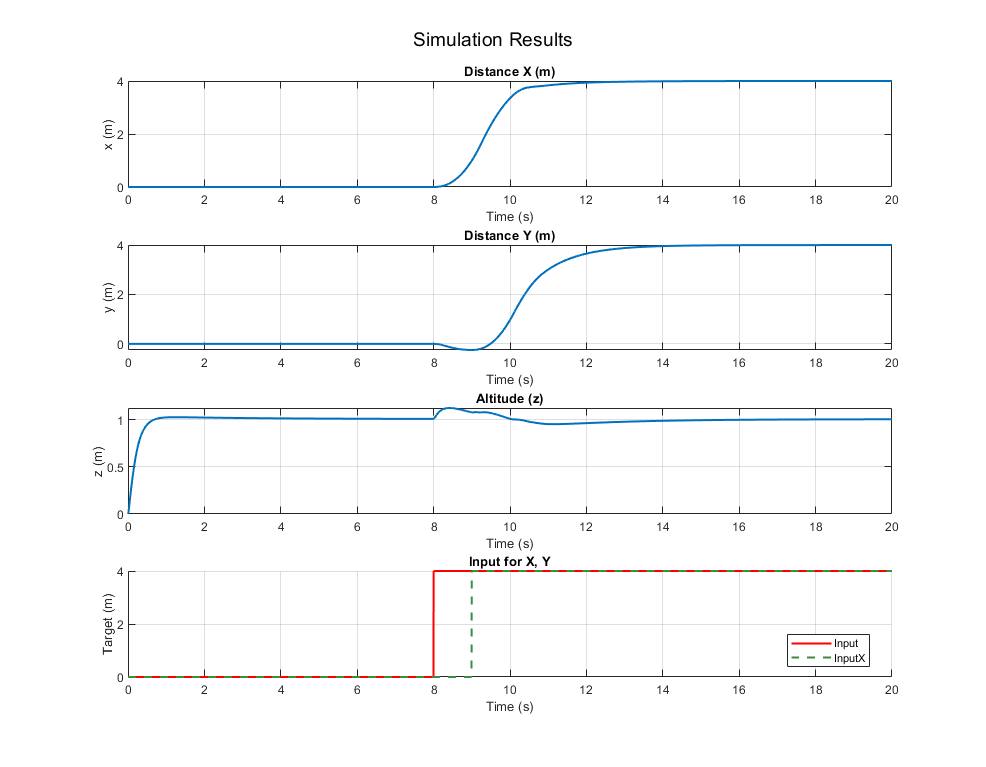
\includegraphics[width=1\textwidth]{DroneResponseCPID_disp_to_follow_psi.png} % Specify image file and width
    \caption{Drone position \& Controller input  } % Image caption
    \label{fig:Drone_Angular_Velocities} % Label for referencing the image
\end{figure}
\newline
Παρατηρούμε πως παρά την αυξημένη πολυπλοκότητα του προβλήματος ελέγχου, οι ελεγκτές μας καταφέρνουν να οδηγήσουν το drone αποτελεσματικά στα σημεία ισορροπίας που θέτουμε ως στόχους. Η επίδραση του ελεγκτή της γωνίας yaw είναι αντιληπτή στο διάγραμμα \ref{fig:Drone_Angular_Velocities_follow_psi}. Συγκεκριμένα βλέπουμε την ταχύτητα των ελίκων να αυξάνεται και να μειώνεται με τέτοιο τρόπο ώστε να μην επηρεάζεται καθόλου το ύψος, δίνοντας την κατάλληλη ταχύτητα στο dronε ώστε να ακολουθήσει την επιθυμητή γωνία. Όταν τελικά ο στόχος της γωνίας σταματάει να μεταβάλεται, παρατηρούμε την αντίθετη συμπεριφορά από το σύστημα ώστε αυτό να πάψει να στρέφεται. 
\newline
\newline
Στο διάγραμμα \ref{fig:Drone_Euler_Angles_follow_psi} φαίνεται πως ο εκλεκτής μας ανταποκρίνεται πολύ γρήγορα και με ελάχιστο overshoot. 
\FloatBarrier
\begin{figure}[H] % 'h' places the image approximately where it appears in the code
    \centering
    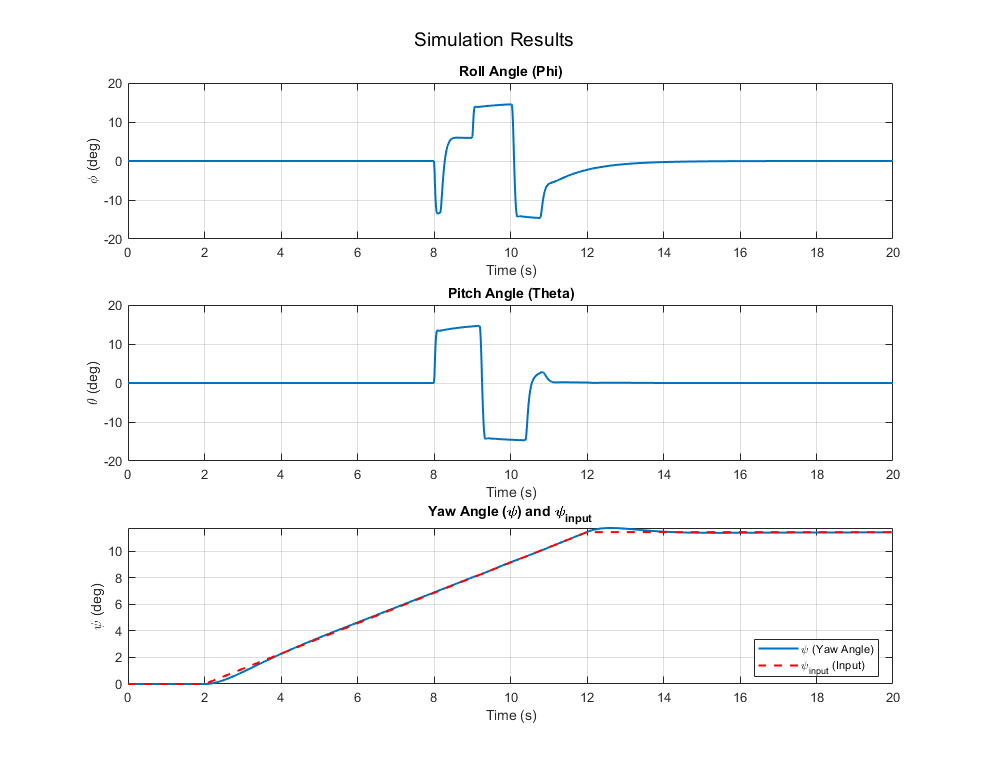
\includegraphics[width=0.84\textwidth]{DroneResponseCPID_to_follow_psi.png} % Specify image file and width
    \caption{Drone Euler angles } % Image caption
    \label{fig:Drone_Euler_Angles_follow_psi} % Label for referencing the image
\end{figure}
\vspace{1em}
\begin{figure}[h!] % 'h' places the image approximately where it appears in the code
    \centering
    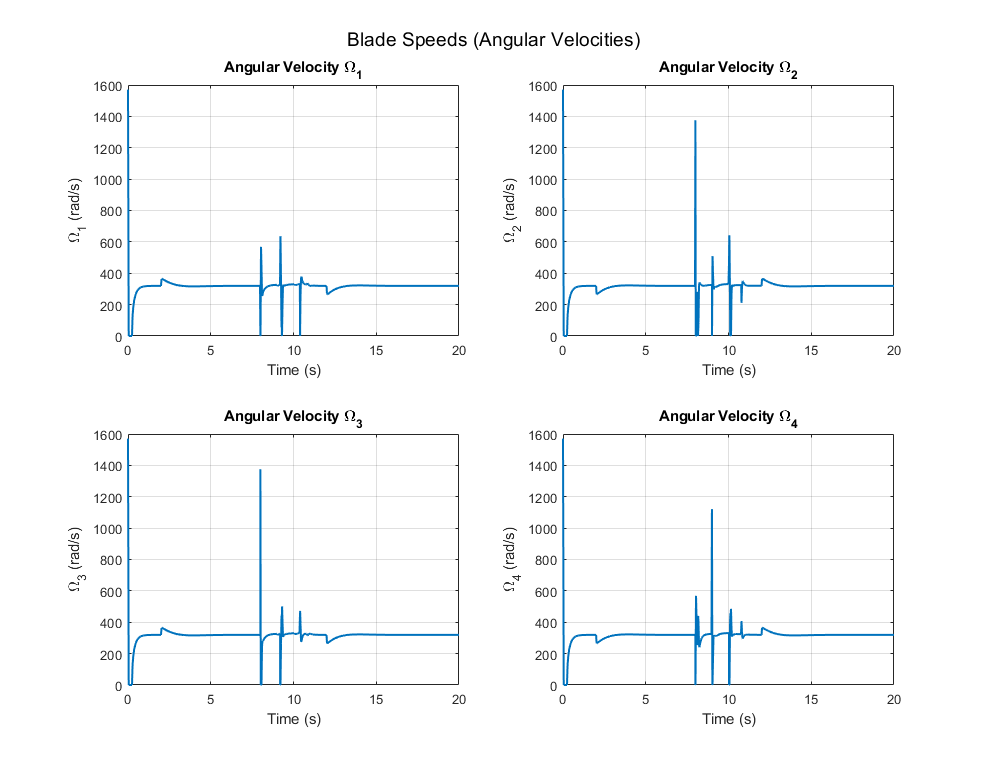
\includegraphics[width=0.84\textwidth]{Drone_Angular_Velocities_to_follow_psi.png} % Specify image file and width
    \caption{Drone angular velocities } % Image caption
    \label{fig:Drone_Angular_Velocities_follow_psi} % Label for referencing the image
\end{figure}
\clearpage
\section{Έλεγχος στο χώρο κατάστασης}
\subsection{Υπολογισμός σημείων ισορροπίας}
Για τον υπολογισμό των σημείων ισορροπίας αρκεί να απαιτήσω να ισχύει η σχέση στην οποία ορίζουμε ώς $s$ το state vector $[x, y, z, \phi, \theta, \psi]$. Επίσης είναι φανερό πως για να ισορροπεί το σύστημα οι γωνίες $\theta$ και $\phi$ πρέπει να είναι 0. Αν αυτό δεν ίσχυε, και το drone είχε ύψος $z > 0$, τότε δεν θα βρισκόταν σε ισορροπία.
\begin{equation}
    \frac{ds}{dt} = 0
\end{equation}
\newline
Οι εξισώσεις κατάστασης λοιπόν, θεωρώντας $\theta = 0$ και $\phi = 0$ γράφονται ώς εξής:
\begin{equation}
    \Ddot{x} = 0
\end{equation}

\begin{equation}
    \Ddot{y} = 0
\end{equation}

\begin{equation}
    \Ddot{z} = 0 \longrightarrow U_1 = mg
\end{equation}


\begin{equation}
    \Ddot{\phi} = 0
\end{equation}

\begin{equation}
    \Ddot{\theta} = 0
\end{equation}

\begin{equation}
    \Ddot{\psi} = 0
\end{equation}
Συμπεραίνουμε λοιπόν πως οποιοδήποτε σημείο στον καρτεσιανό χώρο μπορεί να αποτελέσει σημείο ισορροπίας, αρκεί η συνολική δύναμη ώθησης να είναι ίση με το βάρος του drone.
\subsection{Γραμμικοποίηση γύρω από σημείο ισορροπίας}
Αρχικά, προκειμένου να γραμμικοποιήσουμε το συγκεκριμένο σύστημα, πρέπει να το εκφράσουμε σαν σύστημα διαφορικών εξισώσεων πρώτου βαθμού. Η δυναμική του συστήματος λοιπόν γράφεται ως εξής:
\begin{align*}
\dot{x}_1 &= x_2, \\
\dot{x}_2 &= p_1 x_4 x_6 + p_2 U_2, \\
\dot{x}_3 &= x_4, \\
\dot{x}_4 &= p_3 x_2 x_6 + p_4 U_3, \\
\dot{x}_5 &= x_6, \\
\dot{x}_6 &= p_5 x_2 x_4 + p_6 U_4, \\
\dot{x}_7 &= x_8, \\
\dot{x}_8 &= \left( c_\phi s_\theta c_\psi + s_\phi s_\psi \right) \frac{1}{m} U_1, \\
\end{align*}
\begin{align*}
\dot{x}_9 &= x_{10}, \\
\dot{x}_{10} &= \left( -c_\phi s_\theta s_\psi + s_\phi c_\psi \right) \frac{1}{m} U_1, \\
\dot{x}_{11} &= x_{12}, \\
\dot{x}_{12} &= -g + \left( c_\theta c_\phi \right) \frac{1}{m} U_1,
\end{align*}
Επιλέγουμε να γραμμικοποιήσουμε γύρω από το σημείο ισορροπίας με καρτεσιανές συντεταγμένες $(x,y,z) = (1, 1, 1)$ και γωνίες Euler $(\phi, \theta, \psi) = (0, 0, 0)$. Καθώς λοιπόν που το σύστημα μας έχει πλέον την κατάλληλη μορφή και γνωρίζουμε τα σημεία που μας ενδιαφέρουν, μπορούμε να υπολογίσουμε τους πίνακες A και B του γραμμικού συστήματος πρώτης τάξης από τη σχέση:
\begin{equation}
    \dot{x} = \frac{\partial f(x,u)}{\partial x} (x - x_{ss}) + \frac{\partial f(x,u)}{\partial u} (u - u_{ss})
\end{equation}
\begin{equation}
    A = \frac{\partial f(x,u)}{\partial x},  \quad  B = \frac{\partial f(x,u)}{\partial u}
\end{equation}
Προκύπτει λοιπόν ότι οι πίνακες Α και Β είναι ίσοι με:
\setcounter{MaxMatrixCols}{12}
\begin{equation}
A = 
\begin{bmatrix}
 0 & 1 & 0 & 0 & 0 & 0 & 0 & 0 & 0 & 0 & 0 & 0 \\
0 & 0 & 0 & 0 & 0 & 0 & 0 & 0 & 0 & 0 & 0 & 0 \\
0 & 0 & 0 & 1 & 0 & 0 & 0 & 0 & 0 & 0 & 0 & 0 \\
0 & 0 & 0 & 0 & 0 & 0 & 0 & 0 & 0 & 0 & 0 & 0 \\
0 & 0 & 0 & 0 & 0 & 1 & 0 & 0 & 0 & 0 & 0 & 0 \\
0 & 0 & 0 & 0 & 0 & 0 & 0 & 0 & 0 & 0 & 0 & 0 \\
0 & 0 & 0 & 0 & 0 & 0 & 0 & 1 & 0 & 0 & 0 & 0 \\
0 & 0 & 9.81 & 0 & 0 & 0 & 0 & 0 & 0 & 0 & 0 & 0 \\
9.81 & 0 & 0 & 0 & 0 & 0 & 0 & 0 & 0 & 0 & 0 & 0 \\
0 & 0 & 0 & 0 & 0 & 0 & 0 & 0 & 0 & 1 & 0 & 0 \\
0 & 0 & 0 & 0 & 0 & 0 & 0 & 0 & 0 & 0 & 0 & 1 \\
0 & 0 & 0 & 0 & 0 & 0 & 0 & 0 & 0 & 0 & 0 & 0 \\
\end{bmatrix}
\end{equation}


\begin{equation*}
B = 
\begin{bmatrix}
0 & 0 & 0 & 0 \\
0 & 19.1449 & 0 & 0 \\
0 & 0 & 0 & 0 \\
0 & 0 & 19.1449 & 0 \\
0 & 0 & 0 & 0 \\
0 & 0 & 0 & 35.2858 \\
0 & 0 & 0 & 0 \\
0 & 0 & 0 & 0 \\
0 & 0 & 0 & 0 \\
0 & 0 & 0 & 0 \\
0 & 0 & 0 & 0 \\
1.25 & 0 & 0 & 0 \\
\end{bmatrix}
\end{equation*}

\newpage
\subsection{Υπολογισμός πίνακα μεταφοράς από την είσοδο στην έξοδο (με έξοδους $x, y, z, \psi$)}
Το σύστημα μας είναι ένα MIMO σύστημα (Multiple Input Multiple Output). Συνεπώς δεν ορίζεται μια μοναδική συνάρτηση μεταφορας, αλλά ένας πίνακας συναρτήσεων μεταφοράς από τις εισόδους στις εξόδους. Υπολογίζοντας αυτό τον πίνακα, για το γραμμικοποιημένο σύστημα, μπορούμε να κατανοήσουμε πως επηρεάζει η κάθε είσοδος την έξοδο, καθώς και ποιές είσοδοι επηρεάζουν ποιές εξόδους, κάνοντας ευκολότερο το tuning process κατά τον σχεδιασμό ελεγκτών.

\noindent
Χρησιμοποιώντας τις κατάλληλες συναρτήσεις της MATLAB για να αποφύγουμε λάθη στις πράξεις, υπολογίσαμε τον πίνακα μεταφοράς:
\begin{equation*}
G = 
\begin{bmatrix}
\frac{1.25}{s^2} & 0 & 0 & 0\\
0 & \frac{187.8}{s^4} & 0 & 0\\
0 & 0 & \frac{187.8}{s^4} & 0\\
0 & 0 & 0 & \frac{35.2858}{s^2}\\
\end{bmatrix}
\end{equation*}
\noindent
Για τον παραπάνω πίνακα μεταφοράς ισχύει:
\begin{equation*}
\begin{bmatrix}
    z\\
    y\\
    x\\
    \psi\\
\end{bmatrix} = 
\begin{bmatrix}
\frac{1.25}{s^2} & 0 & 0 & 0\\
0 & \frac{187.8}{s^4} & 0 & 0\\
0 & 0 & \frac{187.8}{s^4} & 0\\
0 & 0 & 0 & \frac{35.2858}{s^2}\\
\end{bmatrix}
\begin{bmatrix}
    U_1\\
    U_2\\
    U_3\\
    U_4\\
\end{bmatrix}
\end{equation*}
Παρατηρούμε πως ο πίνακας μεταφοράς είναι διαγώνιος. Αυτό συμβαίνει καθώς επιλέξαμε να γραμμικοποιήσουμε το σύστημα γύρω από γωνία yaw $\psi = 0$, το οποίο επιτρέπει decoupling των $x$ και $y$. Βλέπουμε επίσης ότι η θέση στον άξονα $x$ επηρεάζεται από το pitch angle, και αντίστοιχα η θέση στον $y$ από το roll angle, δηλαδή η θέση στον $x$ εξαρτάται από την περιστροφή γύρω από τον $y$ και αντίστοιχα η θέση $y$ από την περιστροφή στο $x$. Αυτό είναι μια χρήσιμη παρατήρηση να εκφραστεί και μαθηματικά, γιατί σε συστήματα για το οποία δεν έχουμε τοσο εύκολη εμπειρική κατανόηση, τέτοια πράγματα ίσως να μην είναι τόσο αυτονόητα. Παρατηρούμε επίσης, πως καθώς οι είσοδοι $U_2, U_3$ δεν επηρεάζουν άμεσα τις εξόδους, αλλά τις επηρεάζουν μέσω των γωνιών όπως συζητήσαμε προηγουμένως, χρειάζονται 4 ολοκληρωτές ($s^4$ στον παρονομαστή). Αντίθετα, $U_1, U_4$ επηρεάζουν άμεσα τις μεταβλητές τους οπότε χρειάζονται μόνο 2 ολοκληρωτές.
\newline
\newline
Προφανώς οι παρατηρήσεις αυτές ισχύουν για το γραμμικοποιημένο σύστημα, επομένως γίνεται αντιληπτό ότι το πραγματικό σύστημα δεν θα παρουσιάζει ακριβώς αυτά τα χαρακτηριστικά.
\newpage
\subsection{Σχεδιασμός ελεκτή με LQR και δοκιμή σε συγκεκριμένη πορεία}
Καθώς τώρα έχουμε γραμμικοποιήσει το σύστημα και έχουμε αποκτήσει κάποια κατανόηση για το πως συνδέονται οι έξοδοι με τις εισόδους, μπορούμε να χρησιμοποιήσουμε κλασικά εργαλεία για το σχεδιασμό γραμμικών ελεγκτών σε γραμμικά συστήματα στο χώρο κατάστασης. Συγκεκριμένα θα χρησιμοποιήσουμε έναν LQR, προκειμένου να υπολογίσουμε τα κέρδη του ελεγκτή.
\newline
\newline
Ας περιγράψουμε πρώτα όμως με ένα block diagram το νόμο ελέγχου. Προηγουμένως χρησιμοποιήσαμε 4 cascaded PID ελεγκτές, έναν για κάθε είσοδο. Τώρα λύνοντας την εξίσωση Riccati για επιλεγμένα Q και R matrices, θα καταλήξουμε σε έναν πίνακα κερδών και θα εφαρμόσουμε το νόμος ελέγχου που περιγράφεται από το παρακάτω block diagram.
\begin{figure}[H] % 'h' places the image approximately where it appears in the code
    \centering
    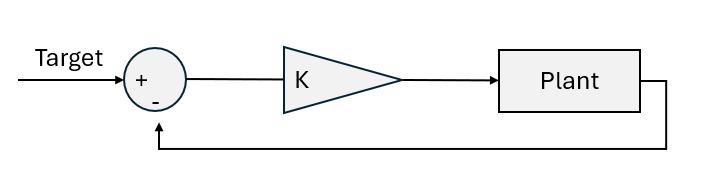
\includegraphics[width=0.84\textwidth]{LQR_Control.png} % Specify image file and width
    \caption{LQR Control law} % Image caption
    \label{fig:LQR_control} % Label for referencing the image
\end{figure}
\noindent
Όπως και στο tuning των PID ελεγκτών, προκειμένου να βρούμε τους καταλληλότερους Q, R πίνακες ακολουθήσαμε μια trial and error διαδικασία. Μετά από πολλές δοκιμές όπου και πάλι ως στόχο είχαμε την γρήγορη απόκριση συστήματος καθώς και την ελαχιστοποίηση απόκλισης από την επιθυμητή κατάσταση καταλήξαμε στους παρακάτω πίνακες:
\begin{equation}
Q = 
\begin{bmatrix}
3 & 0 & 0 & 0 & 0 & 0 & 0 & 0 & 0 & 0 & 0 & 0 \\
0 & 0.01 & 0 & 0 & 0 & 0 & 0 & 0 & 0 & 0 & 0 & 0 \\
0 & 0 & 3 & 0 & 0 & 0 & 0 & 0 & 0 & 0 & 0 & 0 \\
0 & 0 & 0 & 0.01 & 0 & 0 & 0 & 0 & 0 & 0 & 0 & 0 \\
0 & 0 & 0 & 0 & 3 & 0 & 0 & 0 & 0 & 0 & 0 & 0 \\
0 & 0 & 0 & 0 & 0 & 0.1 & 0 & 0 & 0 & 0 & 0 & 0 \\
0 & 0 & 0 & 0 & 0 & 0 & 1 & 0 & 0 & 0 & 0 & 0 \\
0 & 0 & 0 & 0 & 0 & 0 & 0 & 0.2 & 0 & 0 & 0 & 0 \\
0 & 0 & 0 & 0 & 0 & 0 & 0 & 0 & 1 & 0 & 0 & 0 \\
0 & 0 & 0 & 0 & 0 & 0 & 0 & 0 & 0 & 0.2 & 0 & 0 \\
0 & 0 & 0 & 0 & 0 & 0 & 0 & 0 & 0 & 0 & 15 & 0 \\
0 & 0 & 0 & 0 & 0 & 0 & 0 & 0 & 0 & 0 & 0 & 1 \\
\end{bmatrix}
\end{equation}


\begin{equation*}
R = 
\begin{bmatrix}
1 & 0 & 0 & 0\\
0 & 0.1 & 0 & 0\\
0 & 0 & 0.1 & 0\\
0 & 0 & 0 & 0.1\\
\end{bmatrix}
\end{equation*}
\newpage
\begin{figure}[H] % 'h' places the image approximately where it appears in the code
    \centering
    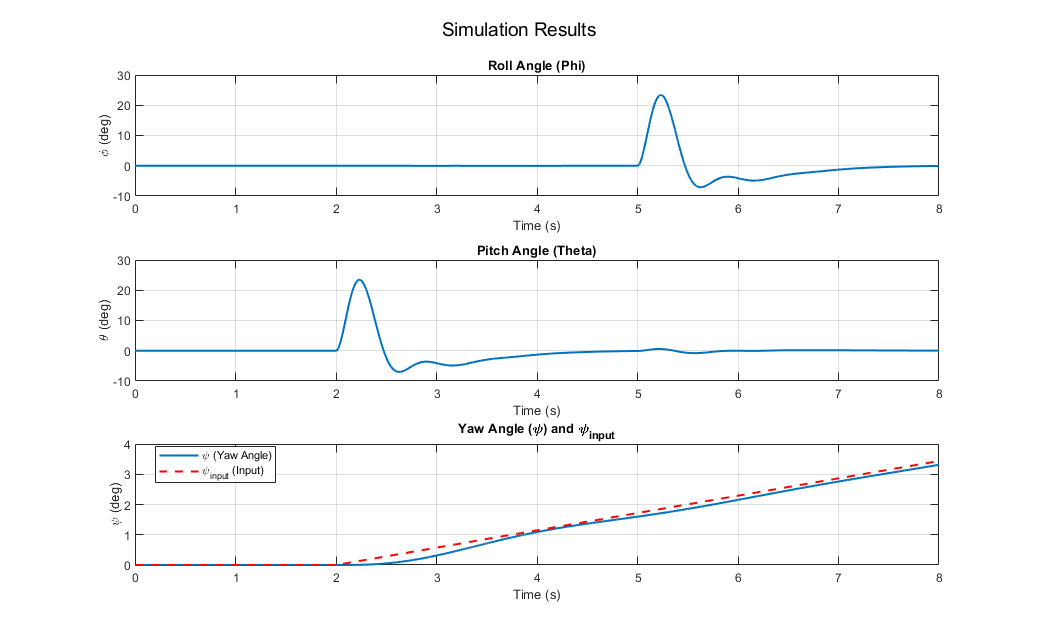
\includegraphics[width=1\textwidth]{LQR_Angles.png} % Specify image file and width
    \caption{LQR controller Euler angle response} % Image caption
    \label{fig:LQR_Angles} % Label for referencing the image
\end{figure}
\begin{figure}[H] % 'h' places the image approximately where it appears in the code
    \centering
    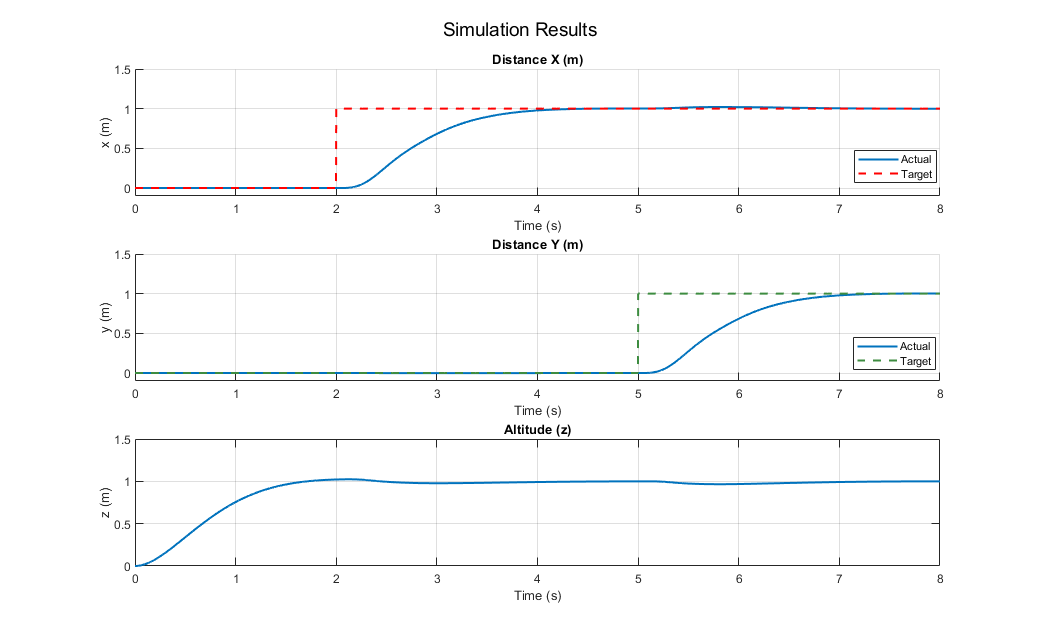
\includegraphics[width=1\textwidth]{LQR_Angles_Disp.png} % Specify image file and width
    \caption{LQR Controller cartesian coordinates} % Image caption
    \label{fig:LQR_Angles_Disp} % Label for referencing the image
\end{figure}
\begin{figure}[H] % 'h' places the image approximately where it appears in the code
    \centering
    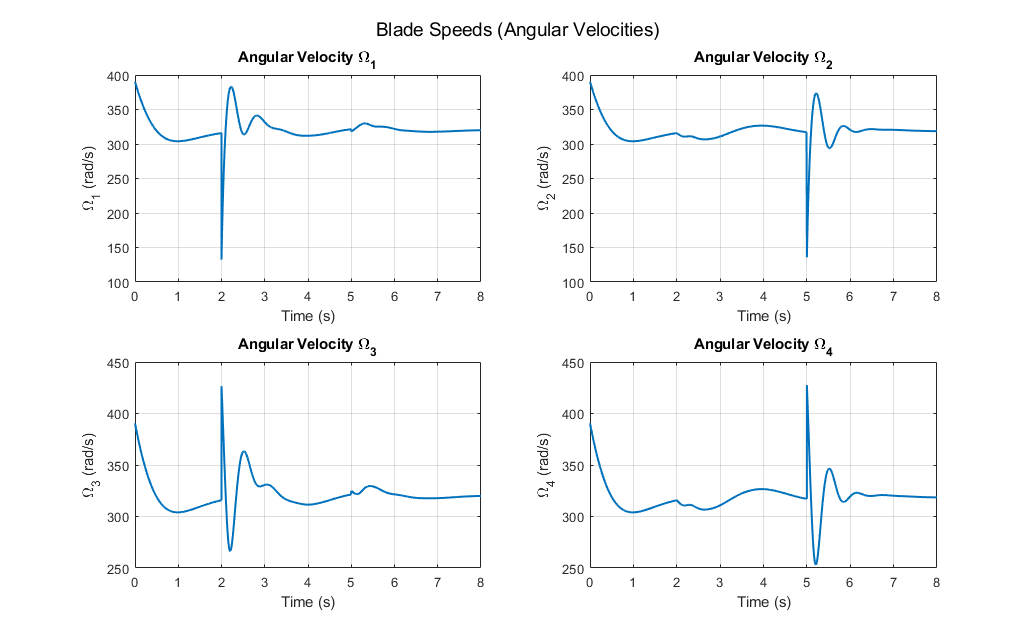
\includegraphics[width=1\textwidth]{LQR_Blade_Speeds.png} % Specify image file and width
    \caption{LQR Controller cartesian coordinates} % Image caption
    \label{fig:LQR_control_blade_speeds} % Label for referencing the image
\end{figure}
\noindent
Είναι φανερό πως ο controller που σχεδιάσαμε με τον LQR, αποδίδει καλύτερα σε σχέση με τους cascaded PID, τόσο και στο πόσο καλά καταφέρνει να ακολουθήσει τον στόχο, χωρίς overshoots, αλλά και από άποψη actuator effort. Αυτό το καταλαβαίνουμε από το διάγραμμα \ref{fig:LQR_control_blade_speeds} καθώς οι αλλαγές στις ταχύτητες είναι πολύ πιο ομαλές, και δεν παρατηρούμε τόσο μεγάλα spikes στις ταχύτητες όπως αυτά που προκαλούν οι PID, που κάνει αυτή τη μέθοδο ελέγχου, και συγκεκριμένα τον ελεγκτή αυτό, προτιμότερη επιλογή για τον έλεγχο ενός physical drone. Σε ένα physical drone, δε θα μπορούμε να επιταχύνουμε με την ίδια ευκολία τους έλικες και επιπλέον, θα επωφεληθούμε από τη χαμηλότερη κατανάλωση ενέργειας. 
\\
\\
\noindent
Τώρα θα σχεδιάσουμε μια συγκεκριμένη τροχιά και θα ζητήσουμε από τον ελεγκτή του drone, να κινήσει το σύστημα πάνω σε αυτή την τροχιά. 
\begin{figure}[H] % 'h' places the image approximately where it appears in the code
    \centering
    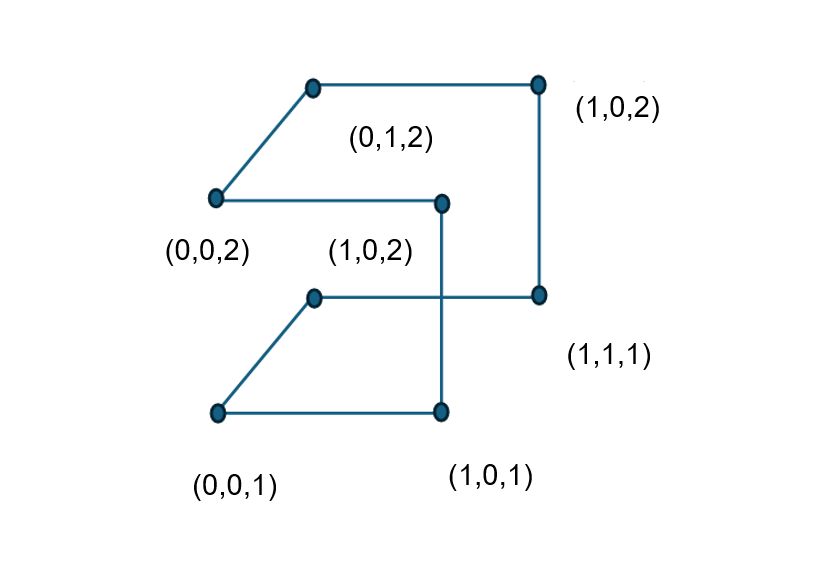
\includegraphics[width=0.5\textwidth]{Trajectory.png} % Specify image file and width
    \caption{Drone desired trajectory} % Image caption
    \label{fig:Trajectory} % Label for referencing the image
\end{figure}
Παρακάτω φαίνεται η απόκριση του συστήματος στην τροχιά:
\begin{figure}[H] % 'h' places the image approximately where it appears in the code
    \centering
    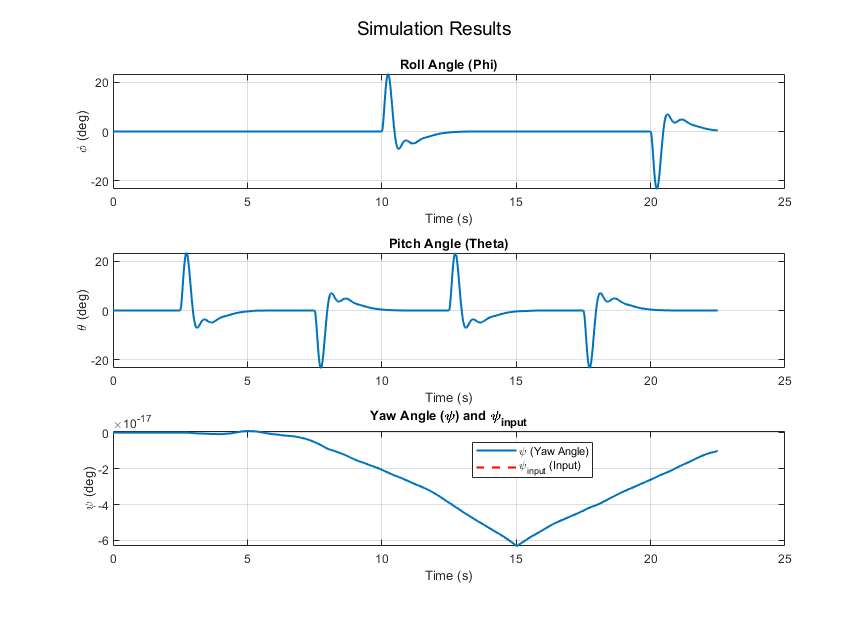
\includegraphics[width=0.95\textwidth]{LQR_Trajectory_Angles.png} % Specify image file and width
    \caption{Drone Euler angles following trajectory described in figure \ref{fig:Trajectory}} % Image caption
    \label{Trajectory_response_angles} % Label for referencing the image
\end{figure}
\begin{figure}[H] % 'h' places the image approximately where it appears in the code
    \centering
    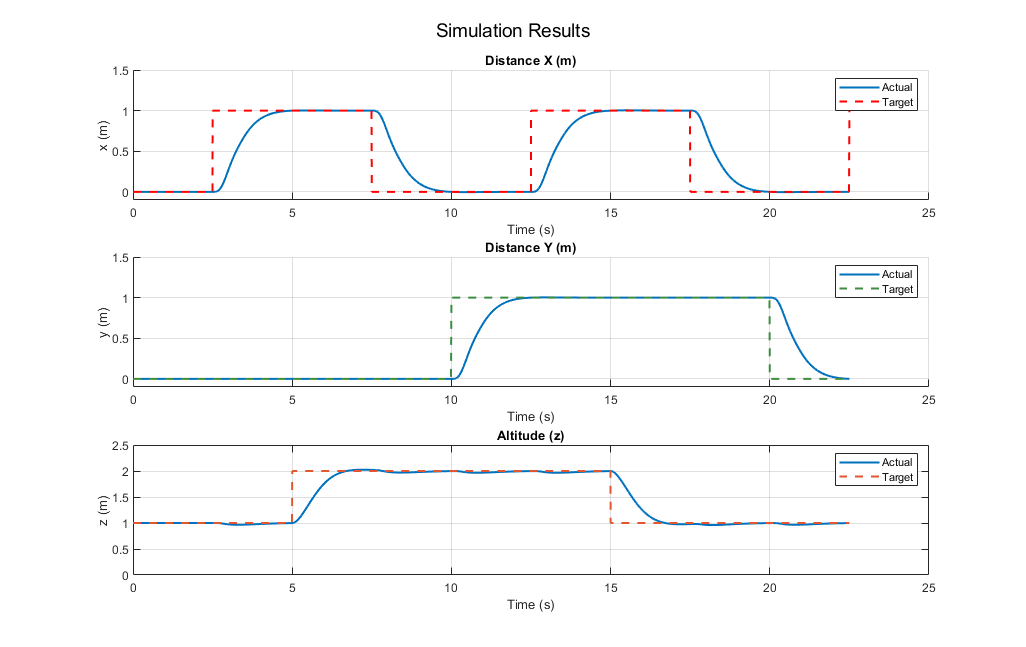
\includegraphics[width=0.99\textwidth]{LQR_T.png} % Specify image file and width
    \caption{Drone response cartesian coordinates \& coordinates of figure \ref{fig:Trajectory}} % Image caption
    \label{fig:Trajectory_response_disp} % Label for referencing the image
\end{figure}
\begin{figure}[H] % 'h' places the image approximately where it appears in the code
    \centering
    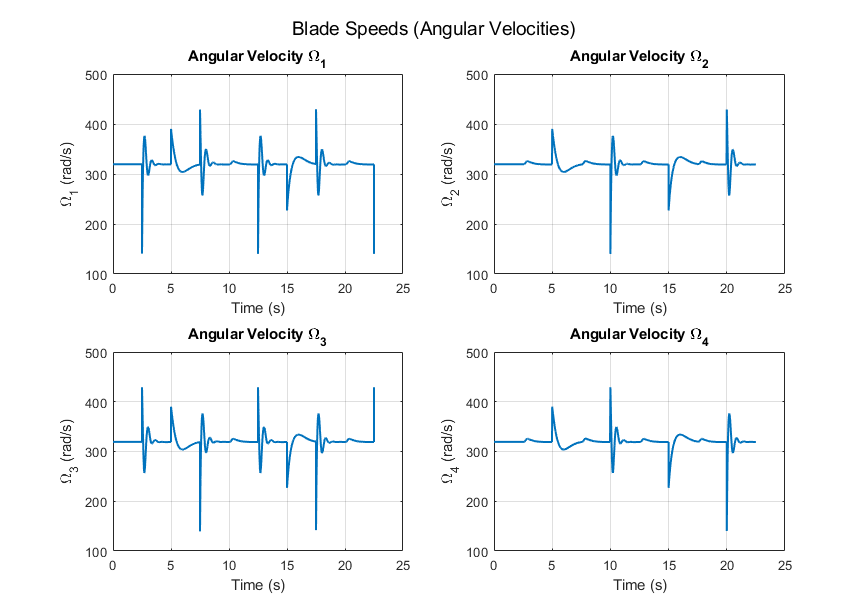
\includegraphics[width=1\textwidth]{LQR_Trajectory.png} % Specify image file and width
    \caption{Drone blade speeds following described in figure \ref{fig:Trajectory} } % Image caption
    \label{fig:LQR_Trajectory_full} % Label for referencing the image
\end{figure}
\noindent
Παρατηρούμε πως o ελεγκτής κρατάει το drone ικανοποιητικά στην τροχιά, χωρίς να έχει αισθητά overshoots η undershoots, και χωρίς να κάνει overwork τους κινητήρες των ελίκων. Στο διάγραμμα \ref{fig:Trajectory_response_blade_speeds} φαίνεται ακριβώς η τροχιά που τελικά ακολουθεί το drone για να γίνει καλύτερα αντιληπτό το performance του ελεγκτή. 
\\
\\
\noindent
Γίνεται για ακόμη μια φορά αντιληπτό πως η προτιμότερη μέθοδος σχεδίασης ελεγκτών είναι μέσω LQR και επίλυσης της αντίστοιχης εξίσωσης Riccati, καθώς και το tuning είναι ευκολότερο, αλλά και η τελική επίδοση του συστήματος είναι καλύτερη. Ειδικά για ένα σύστημα όπως αυτό, όπου έχουμε πολλές μεταβλητές στο χώρο κατάστασης, όταν σχεδιάσαμε τους Cascaded PID ελεγκτές για τις μεταβλητές $x, y$, άρα 4 ελεγκτές, και ακόμη 2 ελεγκτές για τις μεταβλητές $z, \psi$, χρειάστηκε να κάνουμε tune 18 παραμέτρους. Στον LQR ελεγκτή είχαμε 16 παραμέτρους που χρειάστηκαν tuning, που λόγω της ανάθεσης βαρών στο διάνυσμα κατάστασης μέσω του πίνακα Q, κάνει το tuning ιδιαίτερα ευκολότερο απ' ότι του PID.
\\
\\
\noindent 
Σε κάθε περίπτωση, είναι απαραίτητο να αναφέρουμε το σημαντικό πλεονέκτημα της PID μεθόδου, που είναι ιδιαίτερα εύκολη υλοποίηση και προσαρμογή στο μοντέλο. Δε χρειάζεται καμία γραμμικοποίηση η γενικότερα προεπεξεργασία του συστήματος. Παραμένει ένας εύκολος και αξιόπιστος τρόπος να σχεδιάσουμε γρήγορα λειτουργικούς ελεγκτές.

\begin{figure}[H] % 'h' places the image approximately where it appears in the code
    \centering
    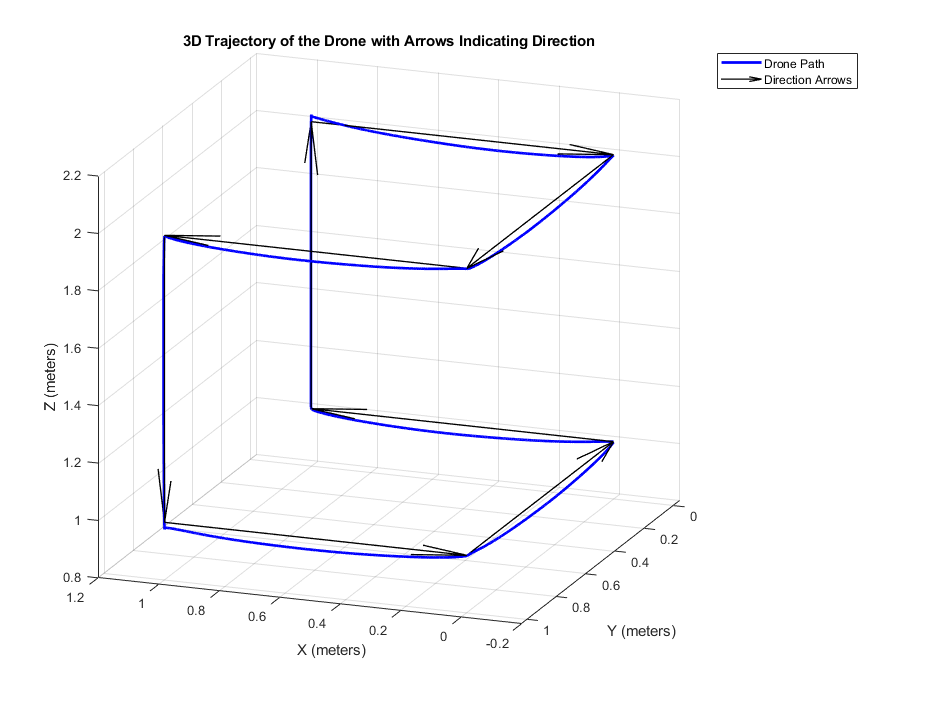
\includegraphics[width=1\textwidth]{Drone_Trajectory.png} % Specify image file and width
    \caption{Drone trajectory response for reference trajectory in figure \ref{fig:Trajectory} } % Image caption
    \label{fig:Trajectory_response_blade_speeds} % Label for referencing the image
\end{figure}
\end{document}
